\documentclass[italian,a4paper]{article}
\usepackage[tight,nice]{units} %unità di misura
\usepackage{babel,amsmath,amssymb,amsthm,graphicx,url}
\usepackage[text={5.5in,9in},centering]{geometry}
\usepackage[utf8x]{inputenc}
\usepackage[T1]{fontenc}
\usepackage{ae,aecompl}
\usepackage[footnotesize,bf]{caption}
\usepackage[usenames]{color}
\usepackage{textcomp}
\usepackage{gensymb}
%\include{pstricks}
\frenchspacing
\pagestyle{plain}
%------------- eliminare prime e ultime linee isolate
\clubpenalty=9999%
\widowpenalty=9999
%--- definizione numerazioni
\renewcommand{\theequation}{\thesection.\arabic{equation}}
\renewcommand{\thefigure}{\arabic{figure}}
\renewcommand{\thetable}{\arabic{table}}
\addto\captionsitalian{%
\renewcommand{\figurename}%
{Grafico}%
}
%
%------------- ridefinizione simbolo per elenchi puntati: en dash
%\renewcommand{\labelitemi}{\textbf{--}}
\renewcommand{\labelenumi}{\textbf{\arabic{enumi}.}}
\setlength{\abovecaptionskip}{\baselineskip}   % 0.5cm as an example
\setlength{\floatsep}{2\baselineskip}
\setlength{\belowcaptionskip}{\baselineskip}   % 0.5cm as an example
%--------- comandi insiemi numeri complessi, naturali, reali e altre abbreviazioni
\renewcommand{\leq}{\leqslant}
%--------- porzione dedicata ai float in una pagina:
\renewcommand{\textfraction}{0.05}
\renewcommand{\topfraction}{0.95}
\renewcommand{\bottomfraction}{0.95}
\renewcommand{\floatpagefraction}{0.35}
\setcounter{totalnumber}{5}
%---------
%
%---------
\begin{document}
\title{Relazione di laboratorio: impedenza in uscita del generatore di funzioni}
\author{\normalsize Ilaria Brivio (582116)\\%
\normalsize \url{brivio.ilaria@tiscali.it}%
\and %
\normalsize Matteo Abis (584206)\\ %
\normalsize \url{webmaster@latinblog.org}
\and %
\normalsize Lorenzo Rossato (579393)\\ %
\normalsize \url{supergiovane05@hotmail.com}}
\date{\today}
\maketitle
\thispagestyle{empty}
%-------
\noindent Impostare il generatore di funzioni in modo che fornisca un uscita sinusoidale di ampiezza $\unit[2]{V}$
picco-picco e frequenza $\unit[20]{kHz}$. Scegliere una resistenza ($R_1$) di valore nominale
$\unit[56]{\ohm}$. 

\begin{center}
 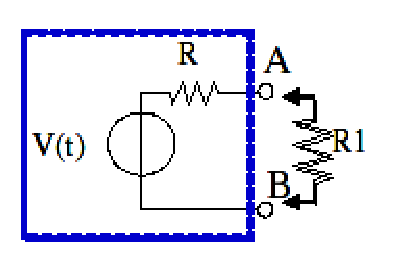
\includegraphics[height=5\baselineskip]{circuito1.eps}
\end{center}
Misurare (con l’oscilloscopio) il valore di tensione tra i punti A e B nelle condizioni di $R_1$ sconnessa
($V_0$) e $R_1$ connessa ($V_{AB}$). Per le due misure si utilizzi il canale 1 dell’oscilloscopio e lo stesso
valore di sensibilità verticale. Ricavare il valore di $R$ dalle misure e calcolarne l’accuratezza. 
La resistenza $R_1$ è stata misurata con il multimetro T110B.
\begin{equation*}
  R_1=\unit[56.0 \pm 0.7]{\ohm}
\end{equation*}
Abbiamo preso tre volte le misure delle differenze di potenziale, perché
l'ampiezza del segnale era leggermente instabile nel tempo. Inoltre tra una
misura e l'altra abbiamo spostato leggermente la manopola dell'ampiezza e
cambiato la persona che eseguiva la misura, per renderle il più possibile
indipendenti. Infine abbiamo determinato la media.
\begin{align*}
V_{0,1}&=\unit[1.34]{V} &\unitfrac[200]{mV}{div}\\
V_{AB}&=\unit[712]{mV}& \unitfrac[200]{mV}{div}\\
V_{0,2}&=\unit[1.34]{V} & \unitfrac[200]{mV}{div}\\
V_{AB}&=\unit[712]{mV}& \unitfrac[200]{mV}{div}\\
V_{0,3}&=\unit[1.46]{V} & \unitfrac[200]{mV}{div}\\
V_{AB}&=\unit[784]{mV}& \unitfrac[200]{mV}{div}
\end{align*}
Resistenza interna del generatore:
\begin{align*}
R_G&=\left(\dfrac{V_0}{V_{AB}}-1 \right)R_1 \\
R_{G,1} &= \unit[49.40 \pm 0.25]{\ohm} \\
R_{G,2} &= \unit[49.40 \pm 0.25]{\ohm} \\
R_{G,3} &= \unit[48.30 \pm 0.24]{\ohm} \\
\end{align*}
possiamo quindi stimare una media: $R_{G,m}=\unit[49.0 \pm 0.15]{\ohm}$. Il
valore riportato nelle specifiche tecniche è $R_{G,0} = \unit[50 \pm
1]{\ohm}$, compatibile con quello misurato.
\end{document}
